\section{Отбор каналов тагирования}
\label{taging}
\subsection{Тагирование $\Lambda_c$}

Для восстановления распадов $\Lambda_c$-барионов и определения импульса недетектируемого нейтрино применяется тагирование по заряду, аромату и барионному числу. Будем предполагать, что $\Lambda_c$ образуется из $\bar{c}$-кварка и подхваченных из вакуума недостающих кварков. В таком случае будем называть систему центромасс $c$-кварка $X_c$, то есть неизвестная очарованная частица, которая фактически может быть не одной, а несколькими частицами сразу.

\begin{figure}[h!]
    \centering
    \begin{tikzpicture}
        \begin{feynhand}
            \vertex [particle] (e) at (-2,1) {$e^-$};
            \vertex [particle] (ae) at (-2,-1) {$e^+$};
            
            \vertex [particle] (photon) at (0,0);
            \vertex (w1) at (1, 0);
            
            \vertex [particle] (c) at (3,1) {$c$};
            \vertex [particle] (anti_c) at (3,-1) {$\bar{c}$};
        
            \propag [fermion] (e) to (photon);
            \propag [anti fermion] (ae) to (photon);
            \propag [photon] (photon) to  [edge label=$\gamma*$]  (w1);
            \propag [fermion] (w1) to (c);
            \propag [anti fermion] (w1) to (anti_c);
        \end{feynhand}
    \end{tikzpicture}
\end{figure}

Для того чтобы определить состав $X_c$, необходимо, чтобы соблюдались законы 
сохранения барионного числа, аромата, заряда, а также 4-импульса. Такая 
технология называется тагированием \textcolor{red}{ссылка на работу}. В 
результате получим, что в $X_c$ будет входить хотя бы один барион и кварки 
$u c d$, а также любые пары $q \bar{q}$. В итоге возможны следующие варианты 
$X_c$. Также важно понимать, что чем больше частиц содержит $X_c$, тем менее 
вероятно событие с такой комбинацией, так как новые частицы требуют 
дополнительных кварковых пар, создание которых требует больше энергии. 
Кроме того, при добавлении новых частиц время работы программы увеличивается 
экспоненциально, так как сложность алгоритма $\mathcal{O}(\prod_n N_n)$ 
(где $N_n$ количестов задетектированных частиц типа $n$ в событии).

В работе рассматриваются $X_c \to \Lambda^{tag}_c; \Lambda^{tag}_c \pi^- \pi^+; \Lambda^{tag}_c \pi^+ \pi^- \pi^+ \pi^-; D^0 p; D^+ p \pi^-; D^{*0} p; D^{*+} p \pi^- $, 
чтобы отличать $\Lambda_c$ котрую тагируемую от тагирующей (той что является продуктом $X_c$), вторую обозначаим как $\Lambda^{tag}_c$.
Каналы распада прочих частиц будем импользовать заведомо изветные самые эффективные каналы, согласно \cite{PDGTablesBar} для барионов и \cite{PDGTablesMes} для мезонов.
\begin{figure}[h]
    \centering
    \begin{tabular}{c|c}
        Particle & Channels \\ \hline
        $D^0$ & $K^- \pi^+; K^- \pi^+ \pi^+ \pi^-; K^- K^+; K^0_s \pi^+ \pi^-; K^0_s \pi^0; K^+ K^- K_s^0$ \\
        $D^+$ & $K^- \pi^+ \pi^+; K^0_s \pi^+; K^0_s \pi^+ \pi^+ \pi^-; K^+ K^- \pi^+$ \\
        $\Lambda^{tag+}_c$ & $pK^-\pi^+; \Lambda^0 \pi^+; \Lambda^0 \pi^+ \pi^0; p K_s^0 \pi^0$ \\
        $D^{*0}$ & $D^0 \pi^0; D^0 \gamma$ \\
        $D^{*+}$ & $D^+ \pi^0; D^0 \pi^+$ \\
        $\pi^0$ & $\gamma \gamma$ \\
        $K_s^0$ & $\pi^+ \pi^-$
    \end{tabular}
    \label{fig:part_channels}
\end{figure}

\subsection{Критерии отбора}

В данном разделе изложены критерии отбора, принятые на основании работы \cite*{BelleDetector2002} и описанном в \ref{mes_mthods}. 
Имея на набор треков и их параметров, надо их классифицировать по типу частици оставившей этот трек. 

\newdot Фотоны классифицированы, но используемые при реконструкции событий, наложим дополнительное ограничение $E_\gamma > 50 \text{ MeV}$, поскольку фотоны с меньшей энергией трудно отличимы тормозных или индуцированных в сичтеме токов, 
что может привести к ошибочной интерпретации их как сигнальных фотонов.

\newdot Идентификация частиц по (PID):

Как уже известно для треков формируется значение правдоподобия $L(p,a)$ 
и в поледствии PID значение $\mathfrak{L}_{p_1/p_2}(a)$, поэтому на треки котрые хотим 
идентифицировать как частицу $p$ наложим следующие ограничения:

\begin{figure}[h]
    \centering
    \begin{tabular}{c|c}
        Гипотеза & Критекрий \\ \hline
        $p \& \bar p$ & $\mathfrak{L}_{p/K} < 0.6; \mathfrak{L}_{p/\pi} > 0.6$ \\
        $K^\pm$   & $\mathfrak{L}_{p/K} < 0.4; \mathfrak{L}_{K/\pi} > 0.6$ \\
        $\pi^{\pm}$ & все заряженные треки, не прошедшие идентификацию по вышеуказанным критериям \\
    \end{tabular}
\end{figure}

\newdot $K_s^0$-мезоны реконструируются по распаду $K_s^0 \to \pi^+ \pi^-$ из кандидатов, отобранных с помощью стандартного инструмента V0finder и собранных в таблице MdstVee2. Критерии отбора следующие:

$$
\left| M_{K_s^0} - M^{real}_{K_s^0} \right| < 30 \text{ MeV}; \ \rho_{K_s^0} > 1 \text{ мм}; \ z_{K_s^0} > 1 \text{ см}; \ \cos \theta_{K_s^0} > 0.99
$$

где $M^{real}_{K_s^0} = 497.611 \text{ MeV}$, $M_{K_s^0}$ — инвариантная масса пионов ($\pi^+ \pi^-$), собранных в $K_s^0$-мезон, $z_{K_s^0}$ и $\rho_{K_s^0}$ — цилиндрические координаты реконструированной вершины распада $K_s^0$-мезона в лабораторной системе отсчёта, а $\cos \theta_{K_s^0}$ — азимутальный угол между импульсом $K_s^0$ и направлением на его вершину распада.

\newdot $\pi^0$ -мезоны восстанавливались в распаде на два фотона, которые в
свою очередь реконструировались по кластерам энерговыделения в ECL.
Критерии отбора:
$$
\abs{M_{\pi^0} - M_{\pi^0}^{real}} < 15 MeV 
$$
После отбора стандартно были установлены погрешности для импульсов фотонов и выполнены фиты в вершину и массу.

\newdot Отбор $D$ -мезонов:

\begin{figure}[h]
    \centering
    \begin{tabular}{c|c}
        $D^0$ & $\abs{M_{D^0} - M^{real}_{D^0}} < 15 MeV$ \\
        $D^\pm$ & $\abs{M_{D^\pm} - M^{real}_{D^\pm}} < 15 MeV$ \\
        $D^{*\pm}$ & $\abs{M_{D^{*\pm}} - M^{real}_{D^{*\pm}}} < 3 MeV$ \\
        $D^{*0}$ & $\abs{M_{D^{*0}} - M^{real}_{D^{*0}}} < 3 MeV$ \\
    \end{tabular}
\end{figure}

Где $M^{real}_{D^\pm} = 1864.83 MeV; M^{real}_{D^0} = 1869.65 MeV; 
M^{real}_{D^{*\pm}} = 2010.26;  M^{real}_{D^{*0}} = 2006.85 MeV$. 
Так де на $D*$-мезоны накладываем ограничение:

\begin{equation}
        \abs{M_{D^*} - M^d_{D}} < 15 MeV
\end{equation}

Где $ M^d_{D}$ --- масса $D$-мезона используемого для кобинации соответствующего. 
$D^*$. Так как ошибка собранного $D^*$ мезона карелирует с собранным 
предврительно $D$-мезоном.

\newdot Для отбора $\Lambda \to p \pi$ требуем 

$$
\abs{ M_{\Lambda_c} - M^{real}_{\Lambda_c} } < 30 \text{ MeV}; 
\ \rho_{\Lambda_c} > 1 \text{ mm}; \ z_{\Lambda_c} > 1 \text{ cm}; 
\ \cos \theta_{\Lambda_c} > 0.99;
\ \mathfrak{L}_{p/K } > 0.6 
$$


\subsection{Итог сбора данных}

Проведя описанную выше реконструкцию событий на $x$ fb из $y$ fb доступных, были получены 
следующие распределения событий. Для аппроксимации распределений был использован 
бинированный алгоритм максимального правдоподобия с предположением о распределении внутри 
бина по Пуассону и общим распределением:

\begin{equation}
    F(x, args) = (1-A)\cdot f_{\text{continuum}} + A \cdot f_{\text{signal}}
\end{equation}

\begin{equation}
    \begin{split}
    f_{\text{continuum}}(x; A_1, \lambda, \mu, \sigma_1, c_0, c_1, c_2, c_3, c_4) = & A_1 \cdot f_{\text{exp}}(x - \mu; \lambda) \\
    & + (1 - A_1) \cdot N(x; 2.65, \sigma_1) \\
    & + c_0 \cdot \tilde T_0(x - \Lambda_c) \\
    & + c_1 \cdot \tilde T_1(x - \Lambda_c) \\
    & + c_2 \cdot \tilde T_2(x - \Lambda_c) \\
    & + c_3 \cdot \tilde T_3(x - \Lambda_c) \\
    & + c_4 \cdot \tilde T_4(x - \Lambda_c)
    \end{split}
\end{equation}
    

\begin{equation}
f_{\text{signal}}(x; A, A_1, \lambda, \mu, \sigma, \sigma_1, c_0, c_1, c_2, c_3, c_4) = \cdot {N}(x; \Lambda_c, \sigma) 
\end{equation}

Определения функций:

1. $f_{\text{exp}}$ Экспоненциальная функция с нормировкой на отрезке $[a, b]$:
\begin{equation}
f_{\text{exp}}(x; \lambda, a, b) = \frac{\lambda e^{\lambda x}}{e^{\lambda b} - e^{\lambda a}}
\end{equation}

2. $\tilde T_0(x - \Lambda_c)$ Поиномы чебышева Чебышева с нормировкой на отрезке $[a,b]$:
\begin{equation}
\tilde T_n(x; a, b) = \frac{T_n(x)}{\text{norm}_n(a, b)}
\end{equation}


\begin{figure}[H]
    \centering
    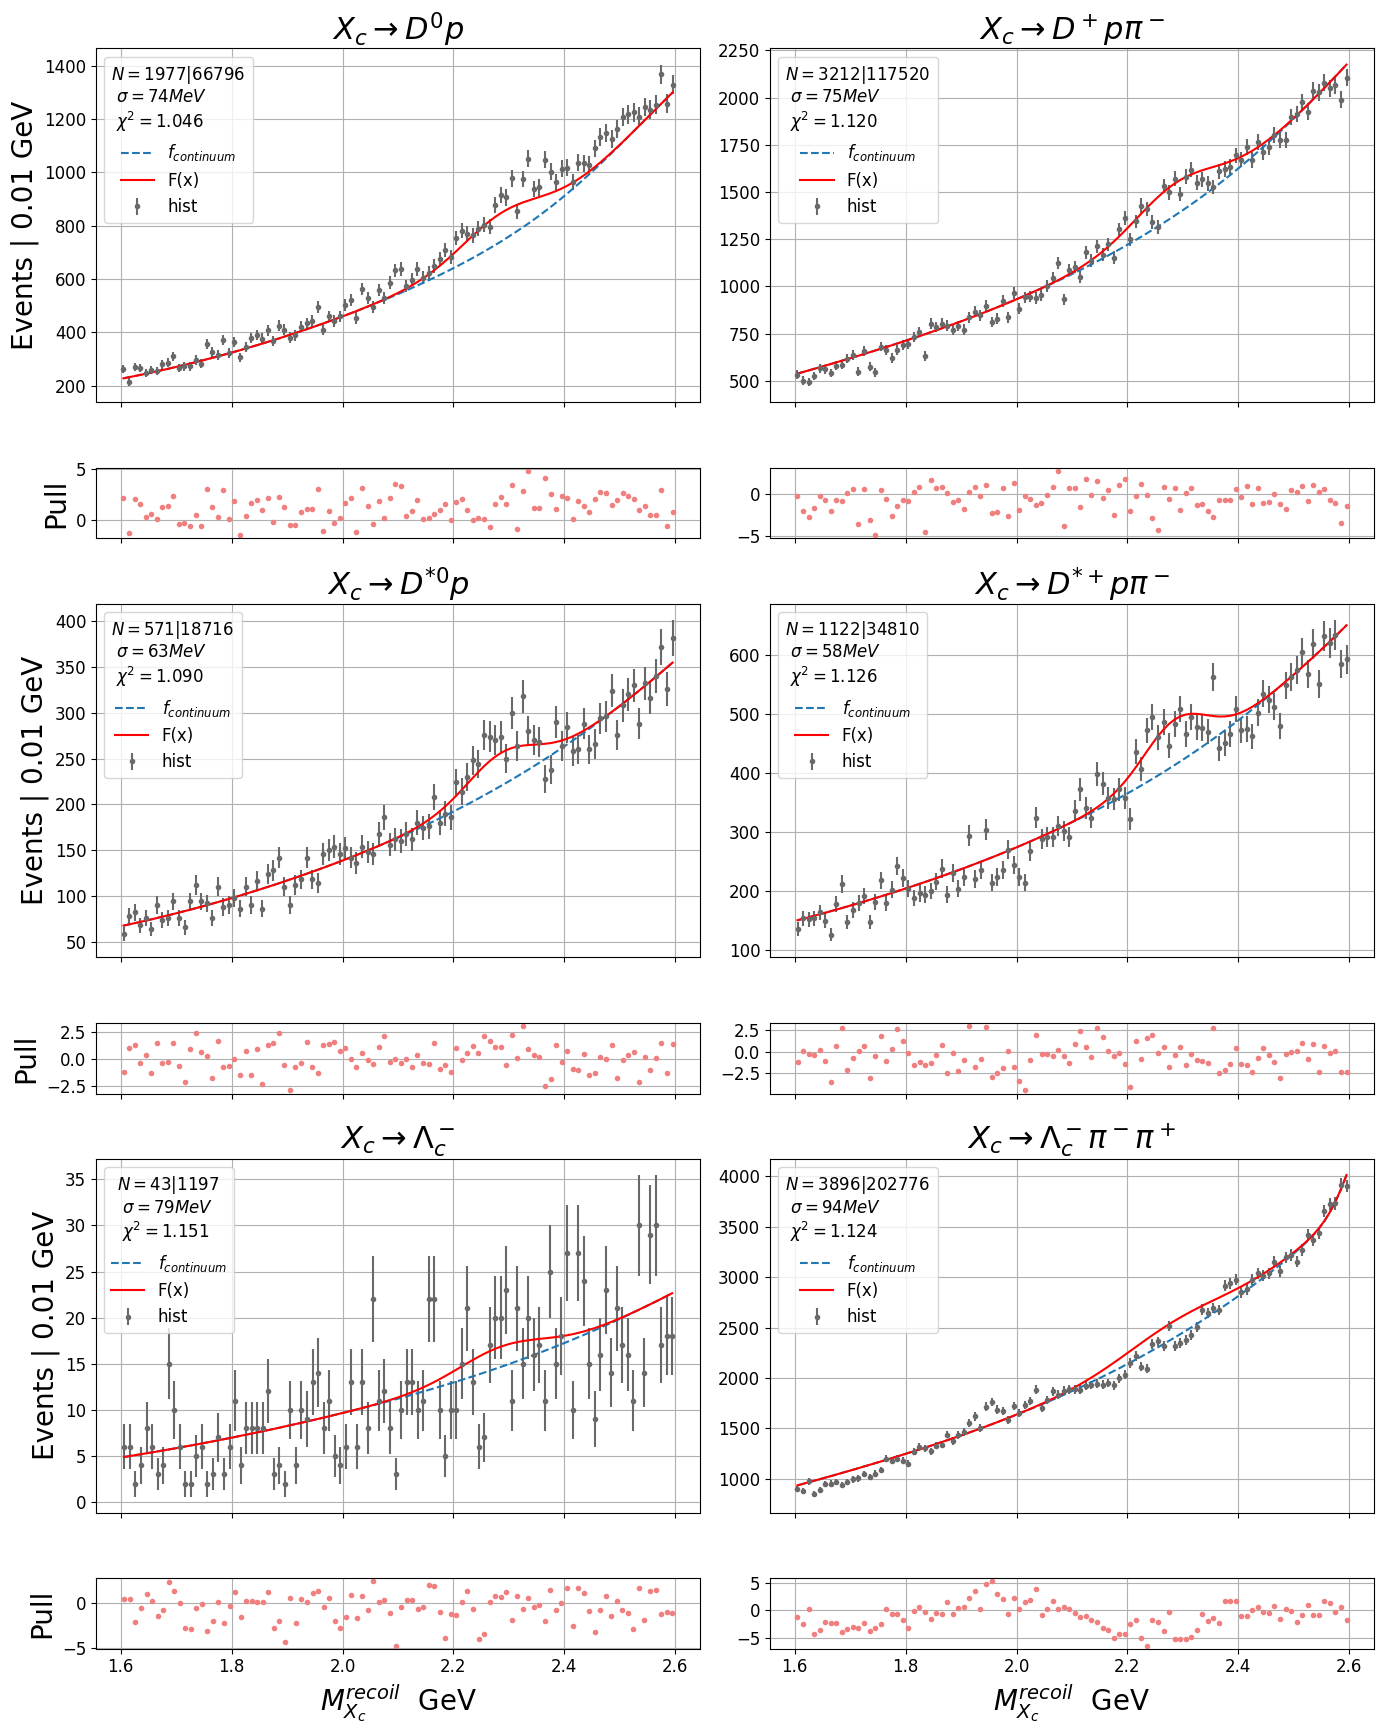
\includegraphics[width=1\linewidth]{img/all_chan_sv.png}
    \caption{Распрееление количества событий по каналам $X_c$.}
\end{figure}

Как мы види канал $X_c \to \Lambda_c^-$ имет очень мальнькое количество событий, 
селедовательно его не разумная трата машиновремени. 
В свою очередь канал $X_c \to \Lambda_c^- \pi^- \pi^+$ очень маленькое отношение 
фона к общему количеству сигнальных событий $\frac{3896}{202776}=0.019$ и очень 
широкое распределение, что в дельнашейшем даст очень большой вклад в погрешность 
расчетов.  

Так же подробное рассмотрение каналов, показало что канал $D^{*0} \to \gamma D^0$, 
тоже имеет очень широкое распределение, что тоже даст нам большую погрешность.

\begin{figure}[H]
    \centering
    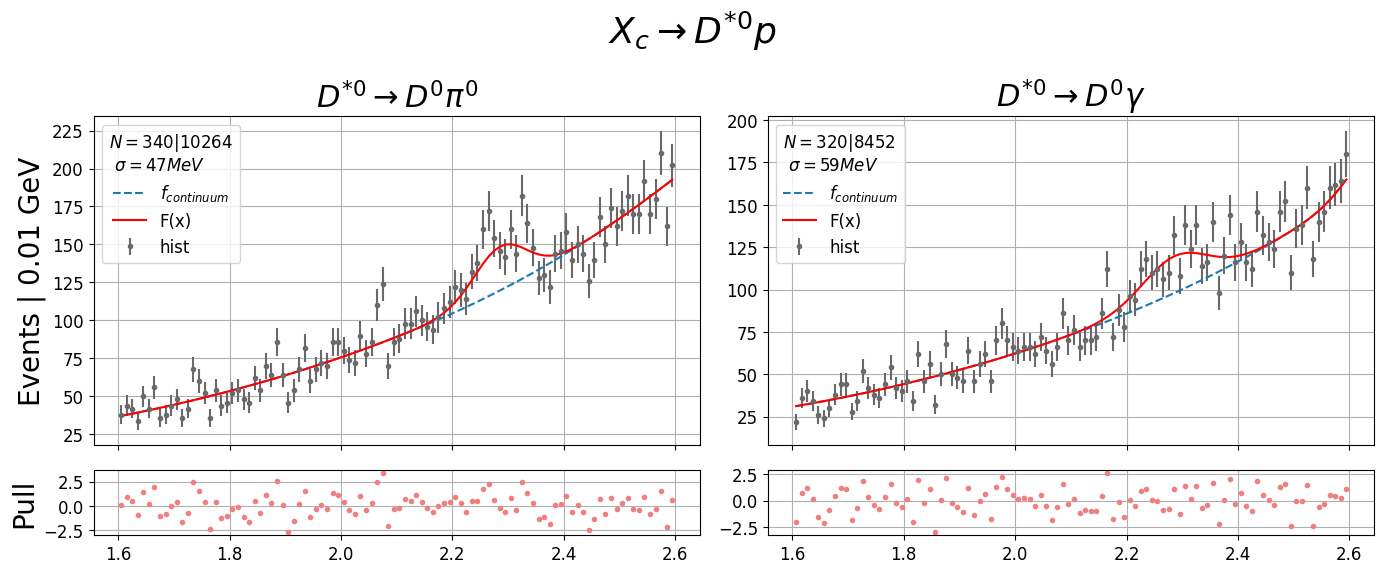
\includegraphics[width=1\linewidth]{img/gamm_pi.png}
    \caption{Распрееление количества событий по каналам $D^{*0}$ в канале $X_c \to D^{*0} p$.}
\end{figure}


\subsection{Итог отбора каналов тагирования}

По итогу педложенных критериев отбора на всех данных собранных Belle удалось, затагировать 
$21828$ и $9860$ событий в каналах $X_c \to D^0 p; D^+ p \pi^-$,  $X_c \to D^{*0} p; D^{*+} p \pi^-$ 
соответственно.

\begin{figure}[H]
    \centering
    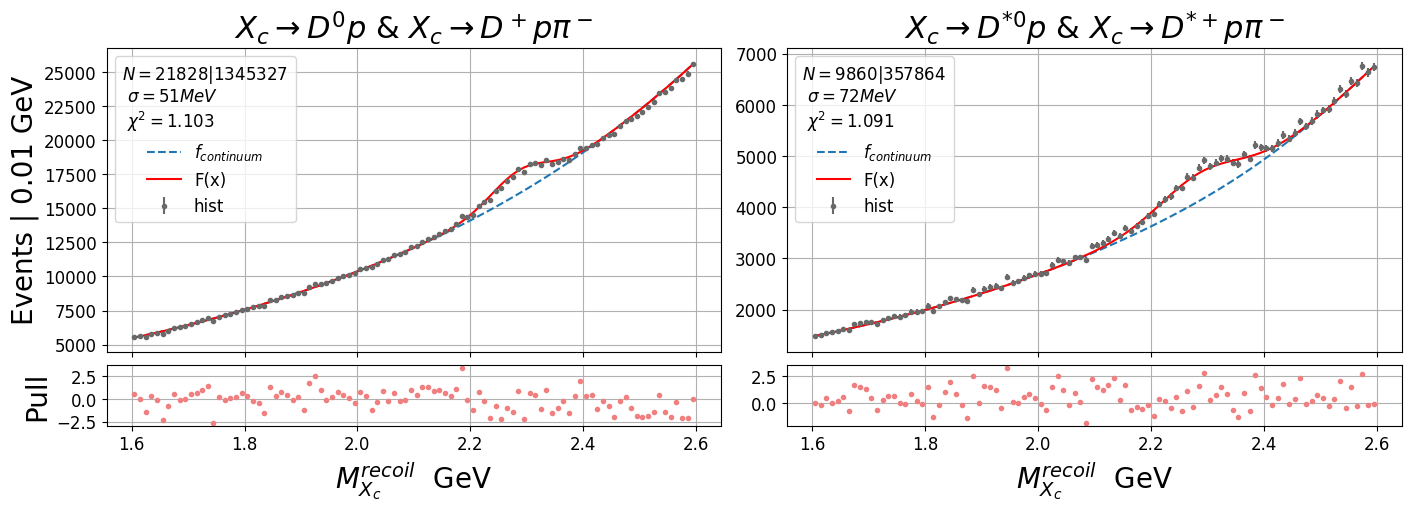
\includegraphics[width=1\linewidth]{img/tag_sum.png}
    \caption{Распрееление количества событий по каналам.}
\end{figure}
